\documentclass[]{sigplanconf}
\usepackage{stmaryrd}
\usepackage{listings}
\usepackage{multirow}
\usepackage{array}
\usepackage{subfig}
%\usepackage{algorithmic}
\usepackage{algorithm}
\usepackage{algpseudocode}
\usepackage{amsmath}
\usepackage{xfrac}
%\usepackage{amsthm}
\usepackage{amssymb}
\usepackage{xspace}
%\usepackage[pdftex]{graphicx}
\usepackage{graphicx}
\usepackage{siunitx}
\usepackage[svgnames,table]{xcolor}
\usepackage{natbib}
\usepackage{adjustbox}
\usepackage{tabularx}
\usepackage{booktabs}
\usepackage{placeins}
\usepackage{hyperref}
\usepackage{tikz}
\usepackage{subfig,epstopdf, todonotes}
\usepackage{makecell}
\usepackage{diagbox}
\usepackage{mathtools}
\usetikzlibrary{automata,positioning}

%\usepackage{amsmath,amsfonts,amssymb,mathtools,url,cite,xspace,graphicx,color,stmaryrd,multirow,verbatim,listings,tikz,pspicture,epstopdf,algorithm,listings,algorithmicx,algorithm,caption,todonotes,algpseudocode}
\hypersetup{
  colorlinks,
	linkcolor={blue!50!black},
	citecolor={blue!50!black},
	urlcolor={blue!80!black}
}
\urlstyle{same}

%\newcommand\comment[1]{\ding{110}\ding{43}\textcolor{red}{#1}}

%\newcommand\code[1]{\textsf{\small #1}}
%\DeclareCaptionType{copyrightbox}
\newcommand\sius[1]{\num[group-separator = {,}]{#1}\si{\micro\second}}
\newcommand\sims[1]{\num[group-separator = {,}]{#1}\si{\milli\second}}
\newcommand\sins[1]{\num[group-separator = {,}]{#1}\si{\nano\second}}
\newcommand\tuple[1]{\langle #1 \rangle}
\providecommand{\abs}[1]{\lvert#1\rvert}

%\newcommand{\mc}[3]{\multicolumn{#1}{#2}{#3}}

\newcommand\Myperm[2][n]{\prescript{#1\mkern-2.5mu}{}P_{#2}}

\input{review}

\begin{document}

\title{Mining timed regular expressions from system traces}

\authorinfo{Greta Cutulenco, Yogi Joshi, Apurva Narayan, and Sebastian Fischmeister}
		   {University of Waterloo, ON, Canada}
		   {\{gcutulen, y2joshi, apurva.narayan, sfischme\}@uwaterloo.ca}

\maketitle

\begin{abstract}

Dynamic behavior of a program can be assessed through examination of events emitted by the program during execution. For the behavior to be correct it\pr must satisfy a set of specified temporal properties. Temporal properties define the order of occurrence and timing constraints on event occurrence. Such specifications are important for safety-critical real-time systems for which a delayed response to an emitted event may lead to a fault in the system. Since temporal properties are rarely specified for programs and due to the complexity of the formalisms, it is desirable to suggest properties by extracting them from traces of program execution for testing, verification, anomaly detection, and debugging purposes. 

We propose a framework for automatically mining properties that are in the form of timed regular expressions (TREs) from system traces. Using an abstract structure of the property, the framework constructs a finite state machine to serve as an acceptor. As part of the framework, we propose two novel algorithms optimized for mining general TREs and a fragment without negation. We analytically derive a speedup for the fragment and confirm the speedup using empirical validation with synthetic traces. Overall, the framework is evaluated on industrial strength safety-critical real-time applications (an deployed autonomous hexacopter system, an commercial vehicle in operation) using traces with more than 1 Million timing-sensitive entries.
\end{abstract}

\section{Introduction}

Temporal behavior of programs is an extensively studied topic\SF{no space before the tilde! fix everywhere}~\cite{lamport1978time, dwyer1999patterns}. % get more sources
Recently, the idea of mining likely temporal properties of programs from system traces has become popular ~\cite{lemieux2015general}.
Critical and commonly occurring behavioral patterns are typically provided to the mining frameworks, which then mine system specifications of that form. The mining techniques identify a set of specifications that are satisfied by traces w.r.t. certain criteria.
Many programs lack formal temporal specifications, and mined specifications are therefore valuable since they can be used for a wide variety of activities in the software development life cycle (SDLC).
These activities include software testing~\cite{dallmeier2010generating}, automated program verification~\cite{kincaid2015automated}, anomaly detection~\cite{christodorescu2008mining}, debugging~\cite{gabel2010online}, etc.
Further, mined specifications can assist automated verification techniques because they provide an easy and user-friendly way to describe a programs' specifications. As argued by Ammons et al.~\cite{DBLP:conf/popl/AmmonsBL02}, automated verification techniques are unlikely to be widely adopted unless cheaper and easier ways of formulating specifications are developed.
Consequently, specification mining has gained significant attention in recent times. Different techniques have been developed for mining specifications from templates expressed using regular expressions, LTL, and other custom formats.

Most of the existing research in the context of mining temporal specifications focuses on a qualitative notion of time, i.e., the specifications describe an \emph{ordering} of events. For example, an LTL specification $\Box(\mathrm{request}\,\rightarrow\,\lozenge \mathrm{response})$ specifies that a \emph{request} event should always be eventually followed by a \emph{response} event. Most state-of-the-art techniques do not take into account a \emph{quantitative} notion of time, i.e., the actual duration of time between events is not considered.
For safety-critical real-time systems, it is important to develop techniques that allow mining of specifications that account for the quantitative notion of time.
For example, specifications for interrupt handlers, which for real-time systems must complete their executions within a set of predefined deadlines. The time constraints are of importance in such a case since a delayed response to an emitted event may lead to a fault in the system.

With the motivation to address the problem of mining specifications with an explicit notion of time, we propose a technique to mine instances of timed regular expression (TRE) templates satisfied by a given system's traces. TREs~\cite{timedregex} extend regular expressions by providing additional operators to specify timing constraints between events. By using a set of common patterns of specifications for LTL and regular expressions, we develop the corresponding patterns for TREs. Further, we use the method proposed by Asarin et al.~\cite{timedregex} to synthesize a timed automaton for a given TRE. The timed automaton is then used as a checker to verify whether traces satisfy the corresponding TRE.

We provide two algorithms for mining instances of TREs from their templates\SF{also mention that you provide complexity analysis}. Both algorithms require a TRE template and system traces as input. The algorithms then use the distinct events from the traces to replace the event variables in the TRE templates with actual events. The resultant \emph{permutations} of the template are TRE instances.
Intuitively, traces are processed against the TRE instances with the help of the timed automaton. Further, we define  \emph{confidence} and \emph{support} as metrics to evaluate the degree to which a TRE instance is satisfied by the traces. The algorithms report only the instances which satisfy the given threshold values of confidence and support.

The first algorithm is designed for TRE templates without a negation operator. The second algorithm processes TRE templates with a negation operator.
We later prove that although both algorithms' execution times are exponential in terms of the number of variables in individual TRE templates, the first algorithm generally runs faster than the second by a certain factor, which depends upon the number of distinct events in a trace and the number of variables in a given TRE template. We also prove that our technique is sound, i.e., a mined specification reported by our algorithms actually satisfies the given thresholds of support and confidence on the provided input traces. Also, our technique is complete, i.e., our algorithms report all TRE instances which comply on given traces w.r.t. the thresholds of support and confidence.

We evaluate our technique on real-world datasets that consist of traces produced by the QNX Neutrino Real-time Operating System~\cite{QNX_RTOS} during various runs of application software on different hardware platforms. We also evaluate the algorithms on the controller area network (CAN)~\cite{Davis2007} traces collected from an automobile during different driving phases. We report the performance of our algorithms on the real-life traces in terms of the execution time. We also demonstrate the scalability and efficiency of our approach by running the implementations on synthesized traces of different sizes with different values of parameters such as the number of distinct events, the total number of events in the traces, and the complexity of the TRE templates.

\noindent The key contributions of this paper include:

\begin{itemize}
\item An efficient technique for extracting temporal properties with time constraints in the form of Timed Regular Expressions (TREs),
\item Two novel algorithms to mine instances of TREs from given system traces. To our knowledge, this is the first technique for mining specifications with an explicit notion of timing constraints.
\item Computational approaches that optimize the extraction of the specified properties for fragments of TREs.
\item An analytic bound on the speedup of the optimization with an empirical validation corroborating the correctness.
\item A feasibility and viability study using traces collected from operating safety-critical real-time systems showing the applicability and scalability of the approach.
\end{itemize}

\section{Background} \label{Background}

\subsection{Timed Regular Expressions}

Regular expressions offer a declarative way to express the patterns for any system property or specification. Every language defined by a regular expression is also defined by a finite automaton ~\cite{book1}. There is a way to convert any regular expression into a non-deterministic automaton, and further to convert from a non-deterministic to a deterministic automaton. We can thus generate a calssical Deterministic Finite Automaton (DFA) for any property expressed as a regular expression.


Classical automata theory handles only the \emph{qualitative} notion of time, i.e. a sequence of events specifies the ordering of events but not the time between occurrence of these events in terms of ``real time". An abstraction of this sort has been found useful for analysis of certain systems [???], whereas many other application domains require more detailed models which include accurate timing information [???]. For example, we might want to modify a formal specification \emph{``a is followed by b"} to a more precise specification with timing constraints \emph{``a is followed by b within $x$ seconds"}. Since our focus lies on real-time safety-critical systems, we need to develop techniques for mining specifications that include the relevant timing information. We use the formalism of Timed Regular Expressions (TREs) for our purpose as it allows for defining explicit timing constraints in the model. We will formally describe our nomenclature.

\newtheorem{defns}{Definition}

\begin{defns}[Trace and event]
The alphabet of events is a finite alphabet of strings. An timed sequence of events is a trace.
\end{defns}

The sequences of events in the trace are ordered by time stamps.
The alphabet of events is defined by the system generating the traces. The events have associated meaning pertaining to the functionality of the system.


\begin{defns}[Timed Regular Expression (TRE) \cite{timedregex}]
Timed regular expressions (TREs) over an alphabet $\Sigma$ (also referred to as $\Sigma$-expressions) are defined using the following families of rules:
\begin{itemize}
  \item  \underbar{a} for every letter a $\in \Sigma$ and the special symbol $\epsilon$ are expressions,
  \item If $\varphi$, $\varphi_1$ and $\varphi_2$ are $\Sigma$-expressions and $I$ is an integer bound interval then $\langle \varphi \rangle_I$, $\varphi_1 \dot \varphi_2$, $\varphi_1 \vee \varphi_2$ and $\varphi^*$ are $\Sigma$-expressions.
\end{itemize}
\end{defns}

The novel features here with respect to untimed regular expressions are the meaning of the atom $\underline{\alpha}$ which represents an arbitrary passage of time followed by an event $\alpha$ and the $\textless \phi \textgreater _I$ operator which restricts the metric length of the time-event sequences in [[$\phi$]] to be in the interval I. It is important to note that we use TREs, as defined above, to provide specification templates.


\begin{defns}[TRE Templates]
A TRE template is a TRE in which all of the atomic propositions are either event variables, events, or time intervals.
\end{defns}

A TRE template is a template for the specifications that we want to mine. We use the term \emph{event variable} to denote a place holder for an event. For example, the TRE template $<0.1>[x,y]$ represents \emph{``0 is always followed by 1 within the time interval [x,y]''}, where 0 and 1 are \emph{event variables} and where $x \le y$ are fixed doubles used in the \emph{time interval}. We use $p$ to denote the number of event variables present in a TRE template. In the given example $p$ is 2.


\begin{defns}[TRE Instance]
Let $\Pi$ be a TRE template. Then, $\pi$ is a TRE instance of $\Pi$ if $\pi$ has a TRE similar to $\Pi$ in structure where all the atomic propositions are events.
\end{defns}

\begin{defns}[Binding]
Let $\Sigma$ be an alphabet of events and let $V$ be a finite set of event variables. Then, a binding is a function $b \colon V \rightarrow \Sigma$
\end{defns}

A TRE instance corresponds to a TRE template and has an identical TRE structure. Applying a binding to the event variables in a TRE template creates a TRE instance corresponding to that binding. The $binding$ is thus a map used to replace event variables with events from the given alphabet.

\subsection{Timed Automata}

Timed automata \cite{Alur:1994:TTA:180782.180519} have been investigated quite rigourously in the recent past. The main motivation for using timed automata is their suitability for modeling time-dependent behavior, and the ability to monitor their reachability \cite{LPY97}. Timed automata are equipped with clocks, making them perfect for modelling and verification of real-time systems' behavior \cite{Alur:1994:TTA:180782.180519}. Classical models like finite automata, Petri-nets, etc., are not suitable since they cannot express such explicit timing constraints natuarally present in real-life systems. Another important property of the timed automata is that the reachability properties are decidable \cite{Alur:1994:TTA:180782.180519}, even though the timed automata have an infinite number of configurations. The main idea behind this result is the construction of a region-automaton, which finitely abstracts the behavior of timed automata in a way that checking reachability in a timed automaton reduces to checking reachability in a finite automaton.

\begin{defns}[Timed Automata \cite{timedregex}]
A timed automaton  $\mathcal{A}$ is a tuple $\langle Q,C,\Delta ,\Sigma, s,F\rangle$ where $Q$ is a finite set of states, $C$ is a finite set of clocks, $\Sigma$ is an input (or event) alphabet, $\Delta$ is a transition relation, $s \in Q$ an initial state and $F \subset Q$ a set of accepting states. The transition relation consists of tuples of the form $\langle q ,\phi ,\rho, a, q' \rangle$ where $q$ and $q'$  are states, $a \in \Sigma \cup \{\epsilon \}$ is a letter, $\rho \subseteq C$ and $\phi$ (the transition guard) is a boolean combination of formulae of the form $(x \in I)$ for some clock $x$ and some integer-bounded interval $I$.
\end{defns}

A clock valuation is a function $v \colon C \rightarrow \mathbb{R}^+$, or equivalently a $|C|$-dimensional vector over $\mathbb{R}^+$. We denote the set of all clock valuations by $\mathcal{H}$ . A configuration of the automaton is hence a pair $(q,v) \in Q \times \mathcal{H}$ consisting of a discrete state (sometimes called “location”) and a clock valuation. Every subset $\rho \subseteq C$ induces a reset function $Reset_\rho : \mathcal{H} \rightarrow \mathcal{H}$ defined for every clock valuation $v$ and every clock variable $x \in C$ as

\begin{equation}\label{timed_automaton}
Reset_\rho v(x) = \begin{cases}
0, & \text{if $x \in \rho$} \\
v(x) &\text{if $x \notin \rho$}
\end{cases}
\end{equation}

$Reset_\rho$ resets all the clocks in $\rho$ to zero and leaves the other clocks unchanged.

\begin{figure}
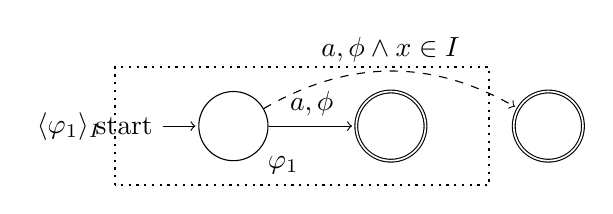
\begin{tikzpicture}[shorten >=1pt,node distance=2cm,on grid,auto]
   \draw[very thick,black](-1.5,0) node[left=1pt,fill=white]{$\langle \varphi_1  \rangle_I$};
   \draw[very thick,black](1,-0.5) node[left=1pt,fill=white]{$\varphi_1$};
   \node[state, initial] (s) {};
   \node[state, accepting] (f) [right=of s] {};
   \node[state, accepting] (f1) [right=of f] {};
   \path[->]
    (s) edge node {$a, \phi$} (f)
        edge [bend left,dashed] node {$a, \phi \wedge x\in I$} (f1);
    \draw[thick,dotted] (-1.5,-0.75) rectangle (3.25,0.75);
\end{tikzpicture}
\caption{Timed Automata from a Timed Regular Expression}
\label{fig:tretoautomata}
\end{figure}


It has been proven that every timed regular language  defined by a generalilzed regular expression can be recognized by a timed automaton \cite{timedregex}. We present a few simple examples of representing TREs using timed automata.

Consider the TRE $\langle \varphi_1  \rangle_I$ and its equivalent timed automaton shown in \ref{fig:tretoautomata}. Within the rectangle, we have the acceptor for $\varphi_1$ with no timing constraints. For the timed operator, a new clock $x$ is introduced and a test $x \in I$ has been added to guard every transition leading to the final state $f$.


Lets further examine the basic idea behind construction of a timed automaton for $\varphi^*$. If the time interval applies to each $\varphi$ separately, then the clocks need to be reset at each new iteration of $\varphi$. On the other hand, if the time interval applies to the whole $\varphi^*$ expression, we need the values of all clocks at each new iteration of $\varphi$ to represent the total time elapsed in the previous iterations. This is achieved by adding a new clock $x$ which is never reset to zero and transitions to the initial state in which all the clocks get the value of $x$.


\subsection{Dominant Properties}

The TRE instances generated by the binding contain every permutation of events in the alphabet within the TRE template. There is thus a total of $\Sigma^p$ possible TRE instances. Generally, we are interested in mining all of the valid TRE instances.
However, these instances contain both interesting and frequently occuring patterns, as well as those that might have been present just a handfull of times in the trace. We thus use a ranking component to reduce the mined set to contain only the dominant instances, or specifications.

First, we will only consider properties that are \emph{valid}~\cite{lemieux2015general}. We express that a binding and its corresponding TRE instance are interesting if the TRE instance holds on each trace, thus $100 \%$ valid. We also use the concepts of support and confidence from ~\cite{lemieux2015general}.

\begin{defns}[Support Potential]
The support of a TRE instance $\pi$ on a trace $t$ is the number of time points of trace $t$ which \emph{could} falsify $\pi$.
\end{defns}

\begin{defns}[Support]
The support of a TRE instance $\pi$ on a trace $t$ is the number of time points of trace $t$ which could falsify $\pi$, but \emph{do not} falsify $\pi$.
\end{defns}

\begin{defns}[Confidence]
The confidence of a TRE instance $\pi$ on a trace $t$ is the ratio of trace support to trace support potential.
\end{defns}

The ranking component we use is a combination of support and confidence. The effectiveness of selecting a meaningful subset of specifications depends on picking a good set of thresholds.

Since the total number of mined TRE instances is often very large in real systems, we would ideally keep the confidence value at $100 \%$. However, the motivation to reduce this threshold slightly is due to the presence of imperfect traces. Traces can be imperfect as a result of dropped events or execution of faulty programs. In such cases, dominant properties may not be perfectly satisfied in the collected traces. Reducing the threshold will thus include dominant properties from imperfect traces.

We will examine different threshold values for both support and confidence and will evaluate best thresholds for reducing all feasible properties to just the dominant and interesting properties.

\section{Approach} \label{Approach}

\subsection{Workflow}

Figure ~\ref{fig:approach} provides a high level overview of the technique we propose for mining temporal properties from system traces.

\begin{figure}[h]
  \centering
  \includegraphics[trim = 1cm 0cm 0cm 0cm,clip = true,width=\linewidth]{figures/Workflow.png}
  \caption{Property Mining Workflow}
  \label{fig:approach}
\end{figure}

The binding function accepts a set of $N$ traces and a TRE template. We use execution traces collected during system runtime. The time-event traces are generated using instrumentation already present in the system and may include network traffic logs, operating system logs, program instrumentation logs, etc. The binding function accepts a set of $N$ logs, where $N \ge 1$. From these logs, the function extracts an alphabet $\Sigma$ of unique events. The TRE template is an abstraction of the desired temporal property, a temporal relationship of interest for the system. The TRE template uses a set $V$ of event variables, where the variables range from $0$ to $p$. The binding function binds the set $V$ to the alphabet of events $\Sigma$ to generate a set of TRE instances.


The timed FSM evaluates the TRE instances on the same set of $N$ traces. The $\Sigma^p$ TRE instances are encoded in the $p$ dimensional incidence matrix that is used by the timed FSM to keep track of state, clocks, and evaluation results. As the timed automaton evaluates each TRE instance on the trace, it updates the success and failure values in the matrix. When the automaton is finished evaluating the TREs on all the traces, it passes the results matrix to the ranker.


The ranker uses the results matrix generated by the timed FSM to calculate the confidence and support values for each TRE instance. The rank criteria are the threshold values for confidence and support that are used to select only the dominant TRE instances. The ranker uses these criteria to filter out any of the instances with confidence and support values below the specified thresholds. Thus, we are left with only the dominant instances, which are the dominant properties or specifications for the system being analyzed.


Let us demonstrate the above workflow through an example. Consider the TRE template (1.\textless0\textgreater[2,5])+, which is a simplified template for the response pattern. The `.' is the concatenation operator and the `+' is the operator for one or more instances of the expression.  The template specifies that some log event $1$ is followed by another log event $0$ within 2 to 5 time units, and this pattern occurs at least once in the execution trace. The property contains two event variables $0$ and $1$, meaning that the value of $p$ is 2. The binding function will bind the events in $\Sigma$ to the template and generate an adjacency matrix for the TRE instances.

The timed FSM iterates over the time event pairs in a trace and at each new event evaluates the relevant TRE instances. Lets assume the matrix contains an entry where $0$ is bound to an event ``send" and $1$ is bound to an event ``receive". The FSM reads in the event ``send" in the trace at time 0. According to the property, if the next event in the trace is \emph{not} ``receive", the FSM will enter an error state and will increase the failure count for this TRE instance to 1 in the matrix.
Similarly, if the next event \emph{is} ``receive", but the time stamp is 6, the failure count would increase.
If the next event is ``receive" and the time stamp is 3, which is within the 2 to 5 interval, then the automaton will enter a final state and will increase the success count for the TRE instance.

Once the entire trace has been processed, the ranker will iterate over the matrix to calculate the confidence and support values for each TRE instance. The ranker will report only the properties that meet the defined thresholds for these metrics.

\subsection{TRE Mining Algorithm}

An intuitive way to evaluate a TRE on a system execution trace is to recursively evaluate the TRE according to its semantics at every line of the trace. A high level description of the steps taken by the proposed algorithm are as follows:

\begin{itemize}
\item \textbf{Representing a TRE} Parse the input TRE template and transform it into a timed automaton.
\item \textbf{Representing a trace} Parse the input trace into a linear array representation where each unique event has its corresponding time and event id, \emph{[time, eventid]}.
\item \textbf{Checking TRE instances over traces} Iterate over the trace and process each time event pair by matching them to the relavant TRE instances. Update the \emph{success} and \emph{reset} for the relevant TRE instances at each trace event.
\end{itemize}

Below, in Algorithm ~\ref{alg:alg_without_neg}, is a detailed description of the above steps in form of pseudo code.

\begin{algorithm}[h]
    \caption{Timed Regular Expression Mining without Negation}
    \begin{algorithmic}[1]
     \Require  Given a trace with $\Sigma$ unique events and a TRE pattern with $p$ event variables
     \Ensure Parse TRE and formulate a finite Timed Automaton $\rightarrow$ A
     \State Initialize an incidence matrix of size $\Sigma^p$
     \State Initialize the \emph{success} and \emph{reset} counters for all permutations in the matrix
     \For {(each unique event $i$ from the trace)}
     \For {(each permutation with event $i$)}
        \State Update the automaton state;
        \State Update the success if A $\rightarrow$ FS;
        \State Update the reset if A $\rightarrow$ ES;
     \EndFor
     \EndFor
     \State Evaluate Support - S
     \State Evaluate Confidence - C
    \end{algorithmic}
\label{alg:alg_without_neg}
\end{algorithm}


\begin{algorithm}[h]
    \caption{Timed Regular Expression Mining with Negation}
    \begin{algorithmic}[1]
     \Require  Given a trace with $\Sigma$ unique events and a TRE pattern with $p$ event variables
     \Ensure Parse TRE and formulate a finite Timed Automaton $\rightarrow$ A
     \State Initialize an incidence matrix of size $\Sigma^p$
     \State Initialize the \emph{success} and \emph{reset} counters for all permutations in the matrix
     \For {(each unique event $i$ from the trace)}
     \For {(each possible permutation)}
        \State Update the automaton state;
        \State Update the success if A $\rightarrow$ FS;
        \State Update the reset if A $\rightarrow$ ES;
   \EndFor
     \EndFor
     \State Evaluate Support - S
     \State Evaluate Confidence - C
    \end{algorithmic}
\label{alg:alg_neg}
\end{algorithm}

In Algorithm ~\ref{alg:alg_without_neg}, $\Sigma$ is the events alphabet and $p$ is the number of event variables in the TRE template without negation. $A$ denotes the timed automaton and $FS$ and $ES$ denote the final and error states of the timed automaton respectively. $S$ and $C$ denote the \emph{support} and \emph{confidence} metrics of the TRE instances on the given trace.

In contrast, Algorithm ~\ref{alg:alg_neg} evaluates the TREs with negation and has a loop to iterate over all possible permutations (see the Discussion for an explanation of the differences in run times of the loops).

\subsection{Temporal Property Patterns}

The proposed technique relies on mining patterns that include timing constraints. Of interest are the most commonly occurring temporal property patterns, as descrbed in ~\cite{evans1}. In order to make use of these patterns, we extend them by transforming them into TRE Property Patterns. Let us assume we have several causing events $P$ to share one effect event $S$. The TRE property patterns are presented in Table~\ref{TRE_Exp}. The properties impose timing constraints on events by adding a time interval $[x, y]$, where $x \le y$ are fixed doubles.

\begin{table}[ht]
  \centering
  \begin{tabular}{|c|c|}
  \hline
  % after \\: \hline or \cline{col1-col2} \cline{col3-col4} ...
  \textbf{Name} & \textbf{TRE}  \\ \hline
  Response      & $[-P]^*;((P;[-S]^*;S \langle x,y \rangle);[-P]^*)^*$        \\ \hline
  Alternating   & $[-P,S]^*;(P;[-P,S]^*;S;[-P,S]^* \langle x,y \rangle)^*$       \\ \hline
  MultiEffect   &  $[-P,S]^*;(P;[-P,S]^*;S;[-P]^* \langle x,y \rangle)^*$     \\ \hline
  MutiCause     &  $[-P,S]^*;(P;[-S]^*;S;[-P,S]^* \langle x,y \rangle)^*$     \\ \hline
  EffectFirst   &  $[-P]^*;(P;[-P,S]^*;S;[-P,S]^* \langle x,y \rangle)^*$      \\ \hline
  CauseFirst    &  $[-P,S]^*;(P;[-S]^*;S;\langle x,y \rangle [-P]^*)^*$       \\ \hline
  OneCause      &  $[-P]^*;(P;[-P,S]^*;S;\langle x,y \rangle [-P]^*)^*$       \\ \hline
  OneEffect     &  $[-P]^*;(P;[-S]^*;S;[-P,S]^* \langle x,y \rangle)^*$       \\ \hline
\end{tabular}
\caption{TRE Property Patterns}\label{TRE_Exp}
\end{table}


\section{Discussion} \label{discussion}

We will examine the follwoing important characteristics of the proposed temporal property mining technique: soundness, completeness, optimality (in terms of space and runtime), and scalability.


\subsection{Sound and Complete}

We argue that the technique we proposed and described in this paper is sound and complete. By sound we mean that a mined specification reported by our algorithms actually satisfies the given thresholds for confidence and support in the provided input traces. This is the case because our algorithm continuously keeps track of the success and reset rates for each TRE instance in the results matrix. The rates are direct results of execution of the acceptor automaton for the TRE on a trace and are used for calculation of the confidence value for the TRE instance. Given that the reported rates and the derived confidence value are valid, it follows that the derived support value is valid as well. Therefore, any mined specification that our algorithms report satisfies the confidence and support constraints.

By characterizing our technique as complete we mean that our algorithms report \emph{all} the mined specifications that comply with the given thresholds for confidence and suport in the provided input traces. Upon reading a time event pair from the trace, our technique examines every TRE instance that can be affected. If the property contains negation, all the TRE instances are examined at every line of the trace. If the property does not contain negation, all TRE instances that can be affected by the trace event are examined. Thus, at every line of the trace, all the relevant TRE instances are evaluated by the timed automaton. Since all the evaluation results are contained within the matrix, the results for every TRE will be considered when evaluating against the confidence and support thresholds. Therefore, the algorithm will report \emph{all} the TRE instances, the mined specifications, that comply with the confidence and support constraints.


\subsection{Memory Requirements}

The proposed temporal property mining technique requires memory space for the multidimensional results matrix, the timed FSM, and the trace contents.

The storage requirements for the matrix are directly influenced by $p$ and $\Sigma$.
We want to encode the matrix to hold the evaluation results of every TRE instance generated by binding the events from $\Sigma$ to the $p$ event variables in the TRE template. There are $\Sigma^p$ possible TRE instances, thus we need $O(\Sigma^p)$ space to hold the acceptor results.

The dimensionality of the matrix grows proportionally to $p$, the number of symbols in the desired property.
Complex properties that encode a relationship between a large number of events will result in higehr values of $p$.
Increasing values of $p$ in tern will result in exponential space growth.
However, the majority of properties of interest represent relationships among a few events only ~\cite{evans1,dwyer1999patterns}.
Therefore, in general, the dimension $p$ of the matrix will remain small.
According to the properties listed in ~\cite{dwyer1999patterns}, the typical property will be constrained to 6 events.

The value of $\Sigma$, on the other hand, affects the size of each dimension.
The number of unique events $\Sigma$ in the trace will depend on the complexity of the program or system.
However $\Sigma$ has a much smaller effect on the growth of the matrix since it only affects the base number in the
exponential space complexity.


Next, we consider the storage requirements for the timed automaton used to evaluate the TRE.
The storage required for the FSM is proportional to the number of its states ~\cite{book1}.
If $n$ is the length of the TRE, then an equivalent NFA has $O(n)$ states and an equivalent DFA has at most $O(\Sigma^n)$ states. Similar to the matrix, complex properties that encode a lot of relationships between events result in exponential space growth for the FSM. However, majority of interesting properties will remain simple ~\cite{dwyer1999patterns}.


Lastly, the storage requirements for the trace are equivalent to the length of the trace, $O(L)$.
Our mining approach examines one time event pair from the trace at a time, without needing to
store any past or future events for context. It also does not perform any changes on the
contents of the trace. Thus the trace is stored only once and never replicated.

%% Discuss optimality & scalability

The proposed technique is thus scalable with the growing trace size $L$ and with the growing event alphabet $\Sigma$. This is important since we have no control over the events and traces generated by real systems. The technique is sensitive to growing values of $p$ and the length of the expressions $n$. However, as we already mentioned, in practice this will not be a concern since properties remain relatively simple.

\subsubsection{Run Time Requirements}

We assess the performance of our temporal property mining technique in terms of the time required to mine a TRE template on a collected system trace $t$ of length $L$. The execution time of the proposed technique differs depending on whether negation is included within the expression. We will consider the execution time of the main loop in Algorithm ~\ref{alg:alg_without_neg} (without negation) and Algorithm ~\ref{alg:alg_neg} (with negation).

\vspace{3mm}

\noindent \textbf{TRE Templates \emph{with} Negation}

Lets first consider the run time of the loop in Algorithm ~\ref{alg:alg_neg} for TRE templates with negation.
When an event variable in the TRE template is negated, the automaton must evaluate nearly all the TRE instances in the matrix.
This is bacause for any negated event variable, we must consider the entire event alphabet minus the event bound to the variable. The satisfiability of any of these TRE instances may be affected.
For the analysis we look at the total number of distinct event sequences to be evaluated.

Consider TRE template \emph{not 0}.
0 can be bound to `b', forming TRE instance \emph{not `b'}. An event `a' in the trace will affect the satisfiability of this TRE instance, thus its automaton is updated. Similarly, satisfiability will be affected for TRE instances that result from bindings with all other event sybols other than `a'.
On the other hand, if 0 is bound to `a', forming TRE instance \emph{not `a'}, and we see an event `a' in the trace, we do not need to update the automaton for the instance. Thus, for $p=1$, we need to evaluate the automaton for $(\Sigma - 1)$ permutations.

For the worst case analysis, we consider TRE templates where all event variables are negated. At any negated event variable in the template we will similarly consider $(\Sigma - 1)$ possibilities. Table ~\ref{Exec-neg} contains the analysis for the first three values of $p$.

\begin{table}[ht]
  \centering
  \begin{tabular}{|c|c|l|}
    \hline
    \textbf{$p$} & \textbf{TRE Tepmlate} & \textbf{Permutations}\\
    \hline
      1 & $\langle \neg 0 \rangle$ & $(\Sigma - 1)$ \\
    \hline
      2 & $\langle \neg 0 . \neg 1 \rangle$ & $(\Sigma - 1)(\Sigma - 1) = (\Sigma - 1)^2$ \\
    \hline
      3 & $\langle \neg 0 . \neg 1 . \neg 2 \rangle$ & $(\Sigma - 1)(\Sigma - 1)(\Sigma - 1)$ = $(\Sigma - 1)^3$\\
    \hline
  \end{tabular}
\caption{Execution Time with Negation} \label{Exec-neg}
\end{table}

In general, for any TRE template, we are sampling $p$ events from an alphabet of size $\Sigma - 1$ with replacement and ordering. This results in $(\Sigma - 1)^p$ possible combinations to be considered in the loop of Algorithm ~\ref{alg:alg_neg}.

The automaton will thus evaluate $O((\Sigma - 1)^p)$ TRE instances for every time-event pair in the trace. Given that the length of the trace $t$ is $L$, the worst case execution time per trace will be $O((\Sigma - 1)^p \cdot L)$.

\vspace{3mm}

\noindent \textbf{TRE Templates \emph{without} Negation}

Next we examine the run time of the main loop in Algorithm ~\ref{alg:alg_without_neg} for TRE templates without negation. This case differs in that only the TRE instances where the bounded event corresponds to that read from the trace needs to be evaluated. We can thus reduce the previous run time by evaluating ony a subset of all TRE instances that contain the trace event. Providing a bound on the worst case execution time relies on an analysis of the subset of TRE instances that contain the observed event.

For the worst case analysis, we consider permutations of $p$ events without repetition and with ordering. One of the event variables will always be bound to the observed trace event. In the Table \ref{Exec-noneg}, we assume that event `a' is observed in the trace and \underline{a} means that the corresponding event variable is bound to event `a'. By \underline{$\neg$ a} we mean an event symbol other than `a' is bound to the event variable. If \underline{$\neg$ a} is used more than once in an event sequence, the chosen events have to be distinct since the permutations are formulated without replacement. Thus, with each such chosen event, the total number of available events decreases by 1. Table ~\ref{Exec-noneg} contains the analysis for the first three values of $p$.

\begin{table}[ht]
  \centering
  \begin{tabular}{|c|c|l|}
    \hline
    \textbf{$p$} & \textbf{TRE Tepmlate} & \textbf{Permutations}\\
    \hline
      1 & $\langle$ 0 $\rangle$ & \underline{a} = 1 \\
    \hline
      2 & $\langle$ 0.1 $\rangle$ &
      \makecell[l]{\underline{a} \underline{$\neg$ a} + \underline{$\neg$ a} \underline{a} \\
      $= (1)(\Sigma - 1) + (\Sigma - 1)(1) = 2(\Sigma - 1)$ } \\
    \hline
      3 & $\langle$ 0.1.2 $\rangle$ &
      \makecell[l]{\underline{a} \underline{$\neg$ a} \underline{$\neg$ a} + \underline{$\neg$ a} \underline{a} \underline{$\neg$ a} + \underline{$\neg$ a} \underline{$\neg$ a} \underline{a} \\
      $= (1)(\Sigma - 1)(\Sigma - 2) +$ \\
      $(\Sigma - 1)(1)(\Sigma - 2) + (\Sigma - 1)(\Sigma - 2)(1) $ \\
      $= 3(\Sigma - 1)(\Sigma - 2) $ } \\
    \hline
  \end{tabular}
\caption{Execution Time with Negation} \label{Exec-noneg}
\end{table}

\begin{sloppypar}
In general, for an arbitrary value of $p$, the run time is ${p \cdot (\Sigma - 1)(\Sigma - 2) \ldots (\Sigma - p + 1)}$.
We can rewrite this as
${p \cdot \frac{(\Sigma - 1)(\Sigma - 2) \ldots (\Sigma - p + 1)(\Sigma - p) \ldots (1)}{(\Sigma - p)(\Sigma - p - 1) \ldots (1)}}$.
This result can be summarized using the expression ${p \cdot \frac{(\Sigma - 1)!}{(\Sigma - p)!}}$ and the permutation notation ${p \cdot \Myperm[(\Sigma - 1)]{(p - 1)}}$.

The automaton will thus evaluate $O(p \cdot \Myperm[(\Sigma - 1)]{(p - 1)})$ TRE instances for every time-event pair in the trace. Given that the length of a trace $t$ is $L$, the worst case execution time per trace will be
$O(p \cdot \Myperm[(\Sigma - 1)]{(p - 1)} \cdot L)$.
\end{sloppypar}

Notice that the approximate relative speedup of Algorithm ~\ref{alg:alg_without_neg} (without negation) as compared to Algorithm ~\ref{alg:alg_neg} (with negation) is $\frac{\Sigma}{p}$. This observation will be assessed through the experimental evaluation in the next section.

%% Discuss optimality & scalability

Generally, scalability of property mining techniques is limited [???].
The techniques tend to scale poorly with the growing size of the input trace $L$. Our technique is optimal in that respect as for both Algorithms the run time grows linearly with the increasing size of $L$. Given that $L \gg \Sigma$ and $L \gg p$, reading each line of the trace at most once is optimal.
Finally, as mentioned earlier, since the majority of interesting properties are not complex, $\Sigma^p$ will remain small in practice.


\section{Evaluation}

In this Section, we demonstrate the performance and scalability of our approach using a set of real system traces and a set of synthetic traces.

The implementation is made using a combination of R and C++ and is made available as an R package \footnote{\url{https://github.com/gretac/ura.git}}. We use an R package `Rcpp'\footnote{\url{http://www.rcpp.org/}} for integration of R and C++ and make use of C++ internally for better performance. Ragel\footnote{\url{http://www.colm.net/open-source/ragel/}} is a framework we used to synthesize Timed Automata for TREs.

We developed TRE property pattern variants, such as shown in Table~\ref{TRE_Exp}, of commonly used patterns of QREs ~\cite{evans1}. By using these TRE variants as TRE templates, we mined TRE instances from real-world system traces: QNX tracelogger and controller area network (CAN) communication traces. We used different thresholds for \emph{support} and \emph{confidence} to uncover interesting TRE instances. Further, to demonstrate the performance and scalability of our approach, we synthesized traces for different configurations w.r.t. the length of traces, number of variables in a TRE template, and the number of distinct events in traces. For the experiments, we used a single eight core machine equipped with the Intel i7-3820 CPU at 3.60 GHz and 31.4 Gb of RAM. The machine runs Ubuntu 14.04 LTS 64 bit.

\subsection{TRE Templates}
The following four TRE templates are used for the evaluation of both real and synthetic traces. These are the first four TRE property patterns listed in Table~\ref{TRE_Exp} and parametrized with a time interval of 0 to 3,000.
\vspace{2mm}

\noindent \textbf{T-1 (response)}: $(\verb!^!P)^*.((\langle P.(\verb!^!S)^*.S\rangle[0, 3000]).(\verb!^!P)^*$

\noindent \textbf{T-2 (alternating)}: $(\verb!^!P,S)^*.((\langle P.(\verb!^!P,S)^*.S\rangle[0, 3000]).(\verb!^!P,S)^*$

\noindent \textbf{T-3 (multi-effect)}: $(\verb!^!P,S)^*.((\langle P.(\verb!^!P,S)^*.S\rangle[0, 3000]).(\verb!^!P)^*$

\noindent \textbf{T-4 (multi-cause)}: $(\verb!^!P,S)^*.((\langle P.(\verb!^!S)^*.S\rangle[0, 3000]).(\verb!^!P,S)^*$


\subsection{Performance Evaluation using Real QNX Traces}

% short description of the traces used for the evaluation
The QNX real time operating system (RTOS) is used in many safety critical systems, such as medical devices, nuclear monitoring systems, vehicles, etc. The QNX RTOS has a very advanced logging facility, \emph{tracelogger}. Tracelogger facilitates detailed tracing of the kernel and user process activity on any system. More specifically, it can log interrupt activity, various states of processes and threads, communication within the system, kernel calls, custom user events, and much more. The logged events give a detailed view into the behavior of the system, but due to the large quantity of the produced information are often difficult to make use of by developers and system designers. These traces are thus a perfect resource for dynamic mining of system properties and specifications.

% Talk about the goals of this portion of the evaluation
For the evaluation we used a set of traces collected from an operational hexacopter loaded with the QNX RTOS and a user control process. Of interest in this portion of the evaluation are the optimal thresholds for support and confidence that would produce a minimal dominant set of specifications that can be assessed by developers or system designers.

% Talk about the results
Table~\ref{TRE-QNX} presents the results of the evaluation. The hexacopter trace used for the evaluation contained 1 million events, with 205 distinct events. We used the four TRE templates, T-1 to T-4, for the evaluation. The interval used in the templates is sufficient for most interesting interactions to complete. The tables report the number of specifications mined by our algorithm given varying values of support and confidence.

It is evident from the results in Table~\ref{TRE1-QNX} that TRE T-1, the response property, occurs infrequently in the trace for a large number of events. Due to an abundance of inter-process communication and system calls within the kernel, this is expected. The other three TREs are more complex and thus appear to be generally satisfied for a smaller number of event combinations.

The results show that higher threshold values for support and confidence result in less specifications being reported. Let's assume that a developer or engineer would be able to assess around 30 specifications per property, more than that would be abundant. Based on the results in Table~\ref{TRE-QNX}, the support threshold should be kept between 10,000 to 50,000 and the confidence threshold should be kept at 0.8 or higher.

\begin{table}[ht]
  \centering

  \subfloat[Results of Mining TRE T-1]{
    \begin{tabular}{|l|c|c|c|c|c|}
      \hline
      \theadfont\diagbox[width=10em]{Support}{Confidence} & \textbf{1} & \textbf{0.9} & \textbf{0.8} & \textbf{0.7} & \textbf{0.6} \\
      \hline
        1 - 1,000         & 0 & 194 & 275 & 324 & 363\\
        1,000 - 5,000     & 0 & 155 & 192 & 211 & 219\\
        5,000 - 10,000    & 0 &  91 &  95 &  98 & 100\\
        10,000 - 50,000   & 0 &  39 &  39 &  40 &  40\\
        50,000 - 80,000   & 0 &  15 &  15 &  16 &  16\\
        80,000 - 300,000  & 0 &   3 &   3 &   3 &   3\\
      \hline
    \end{tabular} \label{TRE1-QNX}
  }

  \subfloat[Results of Mining TRE T-2]{
    \begin{tabular}{|l|c|c|c|c|c|}
      \hline
      \theadfont\diagbox[width=10em]{Support}{Confidence} & \textbf{1} & \textbf{0.9} & \textbf{0.8} & \textbf{0.7} & \textbf{0.6} \\
      \hline
        1 - 1,000         & 0 & 30 & 36 & 41 & 45\\
        1,000 - 5,000     & 0 & 27 & 32 & 36 & 39\\
        5,000 - 10,000    & 0 & 22 & 25 & 28 & 31\\
        10,000 - 50,000   & 0 & 19 & 19 & 21 & 22\\
        50,000 - 80,000   & 0 & 10 & 10 & 11 & 11\\
        80,000 - 300,000  & 0 &  2 &  2 &  2 &  2\\
      \hline
    \end{tabular}
  }

  \subfloat[Results of Mining TRE T-3]{
    \begin{tabular}{|l|c|c|c|c|c|}
      \hline
      \theadfont\diagbox[width=10em]{Support}{Confidence} & \textbf{1} & \textbf{0.9} & \textbf{0.8} & \textbf{0.7} & \textbf{0.6} \\
      \hline
        1 - 1,000         & 0 & 38 & 52 & 67 & 72\\
        1,000 - 5,000     & 0 & 35 & 47 & 60 & 64\\
        5,000 - 10,000    & 0 & 30 & 40 & 50 & 53\\
        10,000 - 50,000   & 0 & 39 & 39 & 40 & 40\\
        50,000 - 80,000   & 0 & 14 & 14 & 16 & 16\\
        80,000 - 300,000  & 0 &  3 &  3 &  3 &  3\\
      \hline
    \end{tabular}
  }

  \subfloat[Results of Mining TRE T-4]{
    \begin{tabular}{|l|c|c|c|c|c|}
      \hline
      \theadfont\diagbox[width=10em]{Support}{Confidence} & \textbf{1} & \textbf{0.9} & \textbf{0.8} & \textbf{0.7} & \textbf{0.6} \\
      \hline
        1 - 1,000         & 0 & 30 & 38 & 45 & 49\\
        1,000 - 5,000     & 0 & 27 & 34 & 39 & 41\\
        5,000 - 10,000    & 0 & 22 & 25 & 29 & 31\\
        10,000 - 50,000   & 0 & 19 & 20 & 22 & 22\\
        50,000 - 80,000   & 0 & 10 & 10 & 11 & 11\\
        80,000 - 300,000  & 0 &  2 &  2 &  2 &  2\\
      \hline
    \end{tabular}
  }
  \caption{Mining TREs on QNX Traces} \label{TRE-QNX}
\end{table}


\subsection{Performance Evaluation using Real CAN Traces}

\begin{table}[ht]
  \centering

  \subfloat[Results of Mining TRE T-1]{
    \begin{tabular}{|l|c|c|c|c|c|}
      \hline
      \theadfont\diagbox[width=10em]{Support}{Confidence} & \textbf{1} & \textbf{0.9} & \textbf{0.8} & \textbf{0.7} & \textbf{0.6} \\
      \hline
        1 - 1,000           & 12 & 398 & 485 & 506 & 510\\
        1,000 - 5,000       & 12 & 331 & 340 & 358 & 362\\
        5,000 - 10,000      & 12 & 130 & 137 & 154 & 156\\
        10,000 - 50,000     & 12 &  39 &  44 &  44 &  44\\
        50,000 - 80,000     & 12 &  15 &  15 &  15 &  15\\
        80,000 - 150,000    &  1 &   1 &   1 &   1 &   1\\
      \hline
    \end{tabular}
    \label{TRE1-CAN}
  }

  \subfloat[Results of Mining TRE T-2]{
    \begin{tabular}{|l|c|c|c|c|c|}
      \hline
      \theadfont\diagbox[width=10em]{Support}{Confidence} & \textbf{1} & \textbf{0.9} & \textbf{0.8} & \textbf{0.7} & \textbf{0.6} \\
      \hline
        1 - 1,000           & 6 & 55 & 102 & 118 & 131\\
        1,000 - 5,000       & 5 & 12 &  15 &  20 &  27\\
        5,000 - 10,000      & 5 & 12 &  15 &  18 &  23\\
        10,000 - 50,000     & 5 & 11 &  14 &  15 &  16\\
        50,000 - 80,000     & 5 & 11 &  11 &  11 &  11\\
        80,000 - 150,000    & 1 &  1 &   1 &   1 &   1\\
      \hline
    \end{tabular}
  }

  \subfloat[Results of Mining TRE T-3]{
    \begin{tabular}{|l|c|c|c|c|c|}
      \hline
      \theadfont\diagbox[width=10em]{Support}{Confidence} & \textbf{1} & \textbf{0.9} & \textbf{0.8} & \textbf{0.7} & \textbf{0.6} \\
      \hline
        1 - 1,000           & 5 & 20 & 63 & 74 & 93\\
        1,000 - 5,000       & 5 & 12 & 15 & 18 & 23\\
        5,000 - 10,000      & 5 & 12 & 15 & 18 & 23\\
        10,000 - 50,000     & 5 & 11 & 14 & 15 & 16\\
        50,000 - 80,000     & 5 & 11 & 11 & 11 & 11\\
        80,000 - 150,000    & 1 &  1 &  1 &  1 &  1\\
      \hline
    \end{tabular}
  }

  \subfloat[Results of Mining TRE T-4]{
    \begin{tabular}{|l|c|c|c|c|c|}
      \hline
      \theadfont\diagbox[width=10em]{Support}{Confidence} & \textbf{1} & \textbf{0.9} & \textbf{0.8} & \textbf{0.7} & \textbf{0.6} \\
      \hline
        1 - 1,000           & 8 & 85 & 194 & 255 & 288\\
        1,000 - 5,000       & 7 & 41 &  55 &  87 &  96\\
        5,000 - 10,000      & 7 & 34 &  47 &  78 &  87\\
        10,000 - 50,000     & 7 & 34 &  41 &  59 &  63\\
        50,000 - 80,000     & 7 & 30 &  30 &  30 &  30\\
        80,000 - 150,000    & 1 &  1 &   1 &   1 &   1\\
      \hline
    \end{tabular}
    \label{TRE4-CAN}
  }
  \caption{Mining TREs on CAN Traces} \label{TRE-CAN}
\end{table}

% short description of the traces used for the evaluation
Controller area network (CAN) bus is the primary communication medium over which the electrical control units (ECU) within a vehicle exchange commands and information. Each message on the network can be distinguished by an associated ID, which is unique per message type. So, for instance, messages that contain the vehile speed will have a unique and unchanging message ID. Messages transmitted on the network also have an associated timestamp. The actual contents of each message are encoded in a manufacturer specific way. Our interest lies in the time and ID of transmitted messages, and not in the exact content of the message. We treat each message ID as an event occuring in the system.

% Talk about the goals of this portion of the evaluation
For the evaluation we collected a set of traces of CAN network activity produced from an idling vehicle with the engine on. Of interest in this portion of the evaluation are the optimal thresholds for support and confidence that would produce a minimal dominant set of specifications that can be assessed by system designers.

% Talk about the results
Table~\ref{TRE-CAN} presents the results of the evaluation. The trace used for the evaluation contained 140 thousand events, with 43 distinct events. We used the four TRE templates, T-1 to T-4, for the evaluation. The interval used in the templates is equivalent as that used previously in the evaluation of QNX traces. The tables report the number of specifications mined by our algorithm given varying values of support and confidence.


It is evident from the results in Table~\ref{TRE1-CAN} that TRE T-1, the response property, occurs infrequently in the trace for a large number of events. This result resembels that we got using the QNX traces. The other three TREs are more complex and thus appear to be generally satisfied for a smaller number of event combinations.


The results show that higher threshold values for support and confidence result in less specifications being reported. Let's agani assume that an engineer would be able to assess around 30 specifications per property. Based on the results in Table~\ref{TRE-CAN}, the support threshold should be kept between 10,000 to 50,000 and the confidence threshold should be kept at 0.9 or higher.

The thresholds required for both QNX and CAN traces are very similar. The number of mined specifications appears to be very sensitive to the size of the time interval in the TREs. This is evident from Table~\ref{TRE-large-CAN}, where the interval in TRE T-1 was set to [0, 6500] and the property was mined on the CAN trace. Comparing Table~\ref{TRE-large-CAN} to Table~\ref{TRE1-CAN} makes it clear that many more properties are mined when the time interval is increased. Therefore, the interval size is the primary reason for the similarity between the derived threshold values.

\begin{table}[ht]
  \centering
  \begin{tabular}{|l|c|c|c|c|c|}
    \hline
    \theadfont\diagbox[width=10em]{Support}{Confidence} & \textbf{1} & \textbf{0.9} & \textbf{0.8} & \textbf{0.7} & \textbf{0.6} \\
    \hline
      1 - 1,000           & 27 & 596 & 694 & 696 & 696\\
      1,000 - 5,000       & 27 & 518 & 548 & 548 & 548\\
      5,000 - 10,000      & 27 & 479 & 508 & 508 & 508\\
      10,000 - 50,000     & 27 & 343 & 357 & 357 & 357\\
      50,000 - 80,000     & 27 & 100 & 100 & 100 & 100\\
      80,000 - 150,000    &  1 &   1 &   1 &   1 &   1\\
    \hline
  \end{tabular}
  \caption{Mining TRE T-1 with interval [0, 6500] on CAN Traces} \label{TRE-large-CAN}
\end{table}

Based on the shown results, we should also note that the TREs are satisfied infrequently for a lot more event combinations in CAN traces than in QNX traces. This is likely a consequence of a smaller event alphabet. CAN traces have a less versatile mix of events than QNX traces, thus a larger number of CAN events may appear to satisfy any particular property. However, the support threshold can be used to remove the effects of alphabet size variation, since only the interesting properties will be satisfied frequently in the traces.

\subsection{Performance Evaluation using Synthesized Traces}

Real system traces are suitable for testing the feasibility and usefullness of our proposed technique. However, they cannot be easily used to demonstrate some important performance and scalability properties of the approach. For instance, in real systems we have little control over the number of distinct events used in the traces and thus cannot control the alphabet size. We also have little control of the exact length of the traces in real systems.


We synthesized a set of traces by varying the following three parameters: the distinct number of events (the size of the events alphabet $\Sigma$), the total number of events (length $L$ of the traces), and the number of variables in TRE templates ($p$ event variables). We used the TRE property patterns listed in Table~\ref{TRE_Exp}.
Below we will describe each setup for evaluating the performance of our mining algorithm, as well as will present the associated results.

\vspace{3mm}

\noindent \textbf{Setup and Results:} We performed the experiment under three different setups. In each of the setups, the value of one of the tree parameters was varied. The values of others were kept constant. We executed each experiment 10 times.


\vspace{3mm}

\noindent \textbf{Setup 1:}
In this first setup, we varied the total number of events in the traces. The number of distinct events was set to 4, and the number of variables in TRE templates was set to 2. The total number of events in the traces were varied exponentially.

The results are shown in Figure~\ref{fig:plot1}. The x axis represents the total number of events in the traces, and the y axis represents the average execution time of our mining algorithm. Note that the measurement of the execution time includes only the processing of trace events (within the main loop of Algorithm~\ref{alg:alg_without_neg}). The measurement does not include the initialization of the algorithm, the overhead of which is constant.

As shown in Figure~\ref{fig:plot1}, the executuon of our mining algorithms grows linearly w.r.t. the total number of events in the trace. For example, the average execution time is 170 milliseconds for processing 0.1 million events.

\vspace{3mm}

\noindent \textbf{Setup 2:}
In this setup, we varied the number of distinct events. There were 10,000 events in total in each trace, and the number of variables in TRE templates was set to 2. As shown in Figure~\ref{fig:plot2}, the x axis represents the number of distinct events in the traces, and the y axis represents the average execution time of our mining algorithm. The figure shows that the execution time increases exponentially with the growing number of distinct events. The average execution time for processing a trace of 10,000 events with 25 distinct events is 594 milliseconds.

\vspace{3mm}

\noindent \textbf{Setup 3:}
Lastly, in this setup, we varied the number of event variables in the TRE templates. The total number of events in the traces was set to 10,000, and the number of distinct events was set to 10. For this setup, the four TRE templates used for setup 1 and 2 were varied to include different numbers of event variables. For the sake of brevity, we do not list these TRE templates.

Figure~\ref{fig:plot3} shows the variation in the average execution time w.r.t. the number of variables in the TRE templates.
It is evident that the average execution time grows exponentially. The average time for processing a trace of 10,000 events with 10 distinct events and a TRE template containing 4 variables is 4156 milliseconds.

%
%\begin{figure*}[ht]
%  \centering
%  \subfloat[Varying Total Number of Events]{
%  \includegraphics[width=\columnwidth]{Plot1.eps}
%  \label{fig:plot1}
%  }
%  \subfloat[Varying Number of Distinct Events]{
%  \includegraphics[width=\columnwidth]{Plot2.eps}
%  \label{fig:plot2}
%  }\\
%  \subfloat[Varying Number of Variables in TRE Templates]{
%  \includegraphics[width=\columnwidth]{Plot3.eps}
%  \label{fig:plot3}
%  }
%  \subfloat[Comparing Execution of Mining Different Classes of TRE templates]{
%  \includegraphics[width=\columnwidth]{TRESyn.eps}
%  \label{fig:plot4}}
%  \caption{Results on Synthesized Traces}\label{Algs_synth}
%\end{figure*}

\subsection{Comparing Algorithm Performance}

Next, we compared the performance of Algorithm ~\ref{alg:alg_without_neg} and Algorithm ~\ref{alg:alg_neg}, where Algorithm ~\ref{alg:alg_neg} considers TRE templates with negation and Algorithm ~\ref{alg:alg_without_neg} considers TRE templates \emph{without} negation. The TRE templates listed in Table ~\ref{TREs_Syn_Comp} were provided as input to the two algorithms when using synthetically generated traces.

\begin{table}[ht]
	\centering
	\begin{adjustbox}{max width=\columnwidth}
		\begin{tabular}{|c|c|}
			\hline
			\textbf{TRE Templates for Algorithm ~\ref{alg:alg_without_neg}} & \textbf{TRE Templates for Algorithm ~\ref{alg:alg_neg}} \\
			\hline
			 $(\langle P.Q.R \rangle [1, 5000])$& $(\langle P.\verb!^!Q^*.Q.\verb!^!R^*.R \rangle [1, 5000])$  \\
			 \hline
		\end{tabular}
	\end{adjustbox}
	\caption{Comparing Algorithm 1 and Algorithm 2}
	\label{TREs_Syn_Comp}
\end{table}

\begin{figure}[ht]
  \centering
  \includegraphics[width=\columnwidth]{Plot1.eps}
  \caption{Varying Total Number of Events}	
  \label{fig:plot1}
\end{figure}

\begin{figure}[ht]
  \centering
  \includegraphics[width=\columnwidth]{Plot2.eps}
  \caption{Varying Number of Distinct Events}	
  \label{fig:plot2}
\end{figure}

\begin{figure}[ht]
  \centering
  \includegraphics[width=\columnwidth]{Plot3.eps}
  \caption{Varying Number of Variables in TRE Templates}
  \label{fig:plot3}
\end{figure}

\begin{figure}[ht]
  \centering
  \includegraphics[width=\columnwidth]{TRESyn.eps}
  \caption{Comparing Execution of Mining Different Classes of TRE templates}
  \label{fig:plot4}
\end{figure}

For evaluation of real system traces we used the TRE patterns T-1, T-2, T-3 and T-4.

Table~\ref{miningOverhead_time} shows the results of the algorithm comparison on real traces generated from a QNX system. The trace used for the evaluation contained 1 million events, with 205 distinct events. It is evident from the figure that mining properties with negation takes approximately 100 times longer than mining properties without negation. This corresponds to the expected speedup of $\frac{\Sigma}{p}$ (see the Discussion section), which in this case is $\frac{205}{2}$.

Table~\ref{miningOverhead_time} also shows the results of the algorithm comparison on real traces generated from a CAN network. The trace used for the evaluation contained 142,866 events, with 43 distinct events. Again, the figure clearly demonstrates that mining properties with negation takes longer than mining properties without negation, in this case 21.5 times longer. This corresponds to the expected speedup of $\frac{43}{2}$.


\begin{table}[ht]
	\centering
	\begin{adjustbox}{max width=\columnwidth}
		\begin{tabular}{|c|c|c|}
			\hline
			\textbf{Real System} & \textbf{Time Without Negation \newline (in seconds)} & \textbf{Time With Negation \newline (in seconds)} \\
			\hline
			 CAN & 1.03 & 21.83 \\
			 \hline
			 QNX & 34.38 & 3498.37\\
			 \hline
		\end{tabular}
	\end{adjustbox}
	\caption{Results for Real System Traces - QNX and CAN}
	\label{miningOverhead_time}
\end{table}


Lastly, Figure~\ref{fig:plot4} shows the results of the comparison on a synthesized trace. The size of the trace used for this experiment was 50,000 events, with 30 distinct events. It is evident from the figure that mining properties with negation takes approximately 12 times longer than mining properties without negation. This result also closely approaches the expected speedup of $\frac{\Sigma}{p}$ (see the Discussion section), which in this case is $\frac{30}{2}$.

% 1) QNX
% Trace Properties:
% Trace Length - 1 million events
% Alphabet Length = 205
% Place Holders in TRE = 2
% Expected Speed up = 205/2 = Approx 100 times as is clear in the plot attached

% 2) CAN
% Trace Properties:
% Trace Length - 142,866 events
% Alphabet Length = 43
% Place Holders in TRE = 2
% Expected Speed up = 43/2 = Approx 21.5 times as is clear in the plot attached





%\begin{figure*}[ht]
%  \centering
%  \subfloat[Comparing Execution on QNX Traces]{
%  \includegraphics[width=\columnwidth]{QNX_Class_ls.eps}
%  \label{fig:plot5}
%  }
%  \subfloat[Comparing Execution on CAN Traces]{
%  \includegraphics[width=\columnwidth]{CAN_Class_ns.eps}
%  \label{fig:plot6}
%  }
%  \caption{Results on Real System Traces}\label{Algs_real}
%\end{figure*}

\section{Conclusion}

The experimental results confirm the asymptotic analysis of our algorithm's complexity, which is described in previous sections. We present two algorithms for mining of TREs in system traces. Our algorithm is scalable to all commonly occuring temporal properties with increasing number of unique events.


%\bibliographystyle{abbrv}
\bibliographystyle{plainnat}
\bibliography{refs}


\end{document}
